
\begin{refsection}
\chapter{Neural network and deep learning}
\minitoc

\section{Neutral network foundations}

\subsection{Approximation theory}

\begin{theorem}\href{https://en.wikipedia.org/wiki/Universal_approximation_theorem}{link}
Let $\phi(\cdot)$ be a nonconstant, bounded, and monotonically-increasing continuous function. Let $I_m$ denote the m-dimensional unit hypercube $[0,1]^m$. The space of continuous functions on $I_m$ is denoted by $C(I_m)$. Then, given any $\epsilon>0$ and any function $f\in C(I_m)$, there exist an integer $N$, real constants $v_i,b_i\in \R$ and real vectors $w_i\in \R^m$, where $i=1,2,...,N$, such that we may define:

$$F(x) = \sum_{i=1}^{N} v_i \psi(w_i^Tx+b_i),$$
as an approximate realization of the function $f$;
$\abs{F(x) - f(x)} < \epsilon$ for all $x\in I_m$. In other words, functions $F(x)$ of the form $$\sum_{i=1}^{N} v_i \psi(w_i^Tx+b_i)$$ are dense(\autoref{ch:functional-analysis:sec:denseSubsetAndApproximation}) in $C(I_{m})$.
\end{theorem}


\begin{remark}[interpretation]
	
\end{remark}

\subsection{Common functions}
\subsubsection{Loss functions}

\begin{definition}[loss functions]\hfill
\begin{itemize}
	\item (square error)
	$$L = \sum_{i=1}^{N} (y_i - \hat{y}_i)^2,$$
	where $N$ is the number of neurons in the output layer.
	\item (Cross entropy)
	$$L = \sum_{i=1}^{N} -\hat{y}_i\ln y_i,$$
where $N$ is the number of neurons in the output layer.
	
\end{itemize}
\end{definition}

\subsubsection{Activation functions}

\begin{definition}[activation functions and derivatives]\hfill
\begin{itemize}
	\item (sigmoid activation function)
	$$g(z) = \frac{1}{1 + \exp(-z)}, \frac{d}{dz}g(z) = g(z)(1 - g(z)).$$
	\item (tanh activation function)
	$$g(z) = \tanh(z), \frac{d}{dz}g(z) = 1 - g(z)^2.$$
	\item (ReLU activation function)
	$$g(z) = \max(0,z), \frac{d}{dz}g(z) =\begin{cases*}
	0, if~ z < 0\\
	1, if~ z\geq 0
	\end{cases*}.$$
	\item (leaky ReLU activation function)
	$$g(z) = \max(0.01z,z), \frac{d}{dz}g(z) =\begin{cases*}
	0.01, if~ z < 0\\
	1, if~ z\geq 0
	\end{cases*}.$$
	
\end{itemize}	
	
\end{definition}

\subsubsection{Output functions}

\begin{definition}[output functions and derivatives]\hfill
Let $x\in \R^H$ denote the \textbf{output vector} of the previous hidden layer before the output layer.	
Let $y\in\R^O$ denote the \textbf{input vector}(after activation) to the output layer. Let $z\in \R^O$ denote the \textbf{output vector} of the output layer and $z_i$ be its individual component. Then 	
	\begin{itemize}
		\item (sigmoid  function) 
		$$z_i  = g(y_i) = \frac{1}{1 + \exp(-y_i)}, \frac{d}{dt}g(t) = g(t)(1 - g(t)).$$
		\item (softmax function) softmax function, $g(x)$, is a function mapping from $\R^H \to [0,1]^O$. The parameter associated with $g(x)$ is a weighting matrix $W = [w_1,w_2,...,w_K]\in \R^{H\times O}$ such that
		$$z_i = g_i(x) = \frac{\exp(x^Tw_i)}{\sum_{k=1}^{K}\exp(x^Tw_i)},i=1,2,...,O.$$
		
		\item (identity function)
		$$z_i  = y_i, i= 1,2,...,O$$
	\end{itemize}	
\end{definition}



\subsection{Training via backpropagation}

\def\layersep{2cm}
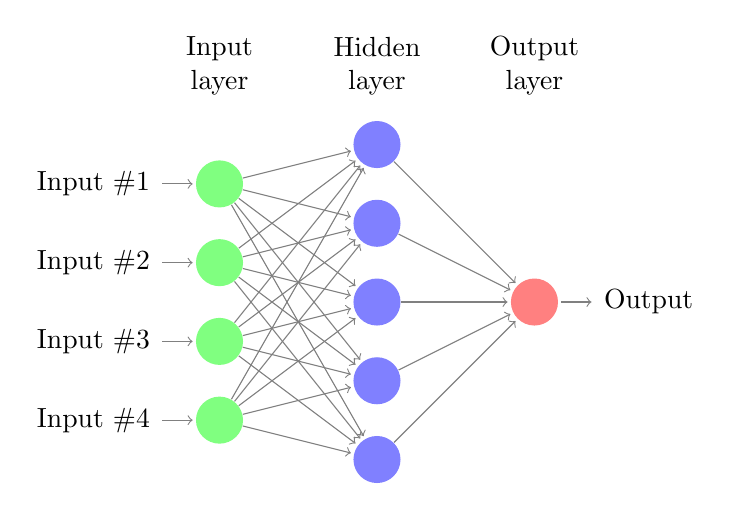
\begin{tikzpicture}[shorten >=1pt,->,draw=black!50, node distance=\layersep]
\tikzstyle{every pin edge}=[<-,shorten <=1pt]
\tikzstyle{neuron}=[circle,fill=black!25,minimum size=17pt,inner sep=0pt]
\tikzstyle{input neuron}=[neuron, fill=green!50];
\tikzstyle{output neuron}=[neuron, fill=red!50];
\tikzstyle{hidden neuron}=[neuron, fill=blue!50];
\tikzstyle{annot} = [text width=4em, text centered]

% Draw the input layer nodes
\foreach \name / \y in {1,...,4}
% This is the same as writing \foreach \name / \y in {1/1,2/2,3/3,4/4}
\node[input neuron, pin=left:Input \#\y] (I-\name) at (0,-\y) {};

% Draw the hidden layer nodes
\foreach \name / \y in {1,...,5}
\path[yshift=0.5cm]
node[hidden neuron] (H-\name) at (\layersep,-\y cm) {};

% Draw the output layer node
\node[output neuron,pin={[pin edge={->}]right:Output}, right of=H-3] (O) {};

% Connect every node in the input layer with every node in the
% hidden layer.
\foreach \source in {1,...,4}
\foreach \dest in {1,...,5}
\path (I-\source) edge (H-\dest);

% Connect every node in the hidden layer with the output layer
\foreach \source in {1,...,5}
\path (H-\source) edge (O);

% Annotate the layers
\node[annot,above of=H-1, node distance=1cm] (hl) {Hidden layer};
\node[annot,left of=hl] {Input layer};
\node[annot,right of=hl] {Output layer};
\end{tikzpicture}


\begin{definition}[feed forward process]
Consider a four layer feed forward neutral network(\autoref{ch:neural-network-and-deep-learning:fig:FourLayerFeedForwardNN}).
Denote input as $x_0$, and parameters $W_1, b_1,W_2, b_2,W_3, b_3$, and activation functions $g_1,g_2,g_3$. Then the feed forward process consists of the following procedures
\begin{align*}
x_1 &= g_1(W_1x_0 + b_1) \\
x_2 &= g_2(W_2x_1 + b_2) \\
x_3 &= g_3(W_3x_2 + b_3)
\end{align*}		
Then the network output is $y=x_3$.
\end{definition}
\begin{figure}
\centering	

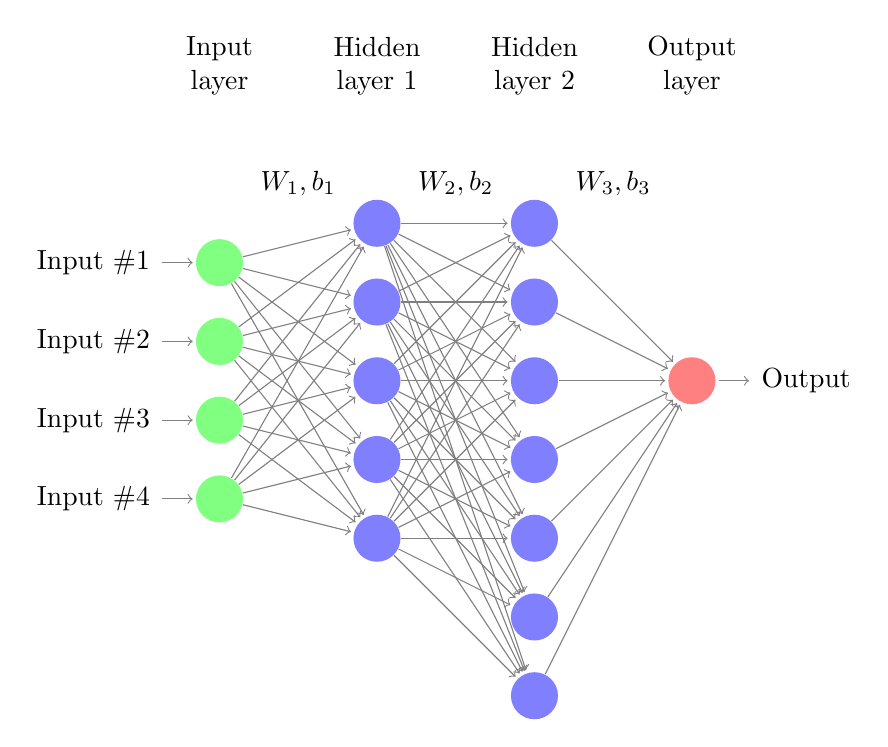
\begin{tikzpicture}[shorten >=1pt,->,draw=black!50, node distance=\layersep]
\tikzstyle{every pin edge}=[<-,shorten <=1pt]
\tikzstyle{neuron}=[circle,fill=black!25,minimum size=17pt,inner sep=0pt]
\tikzstyle{input neuron}=[neuron, fill=green!50];
\tikzstyle{output neuron}=[neuron, fill=red!50];
\tikzstyle{hidden neuron}=[neuron, fill=blue!50];
\tikzstyle{annot} = [text width=4em, text centered]

% Draw the input layer nodes
\foreach \name / \y in {1,...,4}
% This is the same as writing \foreach \name / \y in {1/1,2/2,3/3,4/4}
\node[input neuron, pin=left:Input \#\y] (I-\name) at (0,-\y) {};

% Draw the hidden layer nodes
\foreach \name / \y in {1,...,5}
\path[yshift=0.5cm]
node[hidden neuron] (H1-\name) at (\layersep,-\y cm) {};

% Draw the hidden layer nodes
\foreach \name / \y in {1,...,7}
\path[yshift=0.5cm]
node[hidden neuron] (H2-\name) at (2*\layersep,-\y cm) {};        

% Draw the output layer node
\node[output neuron,pin={[pin edge={->}]right:Output}, right of=H2-3] (O) {};

% Connect every node in the input layer with every node in the
% hidden layer.
\foreach \source in {1,...,4}
\foreach \dest in {1,...,5}
\path (I-\source) edge (H1-\dest);

\foreach \source in {1,...,5}
\foreach \dest in {1,...,7}
\path (H1-\source) edge (H2-\dest);        

% Connect every node in the hidden layer with the output layer
\foreach \source in {1,...,7}
\path (H2-\source) edge (O);

% Annotate the layers
\node[annot,above of=H1-1, node distance=2cm] (hl) {Hidden layer 1};
\node[annot,left of=hl] {Input layer};
\node[annot,right of=hl](h2) {Hidden layer 2};
\node[annot,right of=h2] {Output layer};
\node[annot] at (0.5*\layersep,0) {$W_1, b_1$};
\node[annot] at (1.5*\layersep,0) {$W_2, b_2$};
\node[annot] at (2.5*\layersep,0) {$W_3, b_3$};
\end{tikzpicture}
\caption{A four-layer feed-forward neural network} \label{ch:neural-network-and-deep-learning:fig:FourLayerFeedForwardNN}
\end{figure}

\begin{lemma}[gradient calculation via backpropagation for a four-layer feed forward neutral network]\href{https://sudeepraja.github.io/Neural/}{link}
Consider a four layer feed forward neutral network.
Denote input as $x_0$, and parameters $W_1, b_1,W_2, b_2,W_3, b_3$, and activation functions $g_1,g_2,g_3$.

Denote the forward feeding result as $x_1,x_2,x_3$.

Consider the loss function on the output $x_3$ given by
$$E=\frac{1}{2}\norm{x_3-t}^2,$$
where $t$ is the target value. Then we have
\begin{itemize}
	\item 
	$$\frac{\Pa E}{\Pa W_3} = \delta_3 x_2^T, \frac{\Pa E}{\Pa b_3} = \delta_3,$$
	where $\delta_3 = (x_3-t)\odot g'_3(W_3x_2 +b_3)$.
	\item 	
		$$\frac{\Pa E}{\Pa W_2} = \delta_2 x_1^T, \frac{\Pa E}{\Pa b_3} = \delta_2,$$
	where $\delta_2 = W_3^T\delta_3\odot g'_2(W_2x_1+b_2)$.
	\item 
		$$\frac{\Pa E}{\Pa W_1} = \delta_1 x_0^T, \frac{\Pa E}{\Pa b_1} = \delta_1,$$
	where $\delta_3 = W_2^T\delta_2\odot g'_1(W_1x_0+b_1)$.
\end{itemize}
\end{lemma}
\begin{proof}
(1)	(a)
\begin{align*}
\frac{\Pa E}{\Pa W_3} &= (x_3-t)\frac{\Pa x_3}{\Pa W_3} \\
&= [(x_3-t)\odot g'_3(W_3x_2 + b_3)]\frac{\Pa W_3x_2}{\Pa W_3} \\
&= [(x_3-t)\odot g'_3(W_3x_2+b_3)]x_2^T 
\end{align*}
(b) 
\begin{align*}
\frac{\Pa E}{\Pa b_3} &= (x_3-t)\frac{\Pa x_3}{\Pa b_3} \\
&= [(x_3-t)\odot g'_3(W_3x_2 + b_3)]\frac{\Pa b_3}{\Pa b_3} \\
&= [(x_3-t)\odot g'_3(W_3x_2+b_3)] 
\end{align*}
(2)
(a)
\begin{align*}
\frac{\Pa E}{\Pa W_2} &= (x_3-t)\frac{\Pa x_3}{\Pa W_2} \\
&= [(x_3-t)\odot g'_3(W_3x_2 + b_3)]\frac{\Pa W_3x_2}{\Pa W_2} \\
&= \delta_3\frac{\Pa W_3x_2}{\Pa W_2} \\
&= W_3^T\delta_3\frac{\Pa x_2}{\Pa W_2} \\
&= W_3^T\delta_3\odot g_2'(W_2x_1+b_2)]\frac{\Pa W_2x_1}{\Pa W_2} \\
&= \delta_2x_1^T
\end{align*}
(b)
\begin{align*}
\frac{\Pa E}{\Pa b_2} &= (x_3-t)\frac{\Pa x_3}{\Pa b_2} \\
&= [(x_3-t)\odot g'_3(W_3x_2 + b_3)]\frac{\Pa W_3x_2}{\Pa b_2} \\
&= \delta_3\frac{\Pa W_3x_2}{\Pa b_2} \\
&= W_3^T\delta_3\frac{\Pa x_2}{\Pa b_2} \\
&= W_3^T\delta_3\odot g_2'(W_2x_1+b_2)]\frac{\Pa b_2}{\Pa b_2} \\
&= \delta_2
\end{align*}
(3)
(a)
\begin{align*}
\frac{\Pa E}{\Pa W_1} &= (x_3-t)\frac{\Pa x_3}{\Pa W_1} \\
&= [(x_3-t)\odot g'_3(W_3x_2 + b_3)]\frac{\Pa W_3x_2}{\Pa W_1} \\
&= \delta_3\frac{\Pa W_3x_2}{\Pa W_1} \\
&= W_3^T\delta_3\frac{\Pa x_2}{\Pa W_1} \\
&= W_3^T\delta_3\odot g_2'(W_2x_1+b_2)]\frac{\Pa W_2x_1}{\Pa W_1} \\
&= \delta_2 \frac{\Pa W_2x_1}{\Pa W_1} \\
&= W_3^T\delta_2\odot g_1'(W_1x_0+b_1)]\frac{\Pa W_1x_0}{\Pa W_1} \\
&= \delta_1 x_0^T 
\end{align*}
(b)
\begin{align*}
\frac{\Pa E}{\Pa W_1} &= (x_3-t)\frac{\Pa x_3}{\Pa W_1} \\
&= [(x_3-t)\odot g'_3(W_3x_2 + b_3)]\frac{\Pa W_3x_2}{\Pa W_1} \\
&= \delta_3\frac{\Pa W_3x_2}{\Pa W_1} \\
&= W_3^T\delta_3\frac{\Pa x_2}{\Pa W_1} \\
&= W_3^T\delta_3\odot g_2'(W_2x_1+b_2)]\frac{\Pa W_2x_1}{\Pa W_1} \\
&= \delta_2 \frac{\Pa W_2x_1}{\Pa W_1} \\
&= W_3^T\delta_2\odot g_1'(W_1x_0+b_1)]\frac{\Pa b_1}{\Pa b_1} \\
&= \delta_1 
\end{align*}
\end{proof}


\begin{theorem}[gradient calculation via backpropagation for a multiple-layer feed forward neutral network]\href{https://sudeepraja.github.io/Neural/}{link}

Consider a multi-layer feed forward neutral network with $L$ layers.
Denote input as $x_0$, and parameters $W_1, b_1,W_2, b_2,..., W_L, b_L$, and activation functions $g_1,g_2, ... , g_L$.

Denote the forward feeding result as $x_1,x_2,...,x_L$.

Consider the loss function on the output $x_3$ given by
$$E=f(x_3).$$

Then it follows that
$$\frac{\Pa E}{\Pa W_i} = \delta_i x_{i-1}^T, \frac{\Pa E}{\Pa b_i} = \delta_i, i=1,2,...,L, $$
where
\begin{align*}
\delta_L = \frac{\Pa E}{\Pa x_L}\odot g'_L(W_Lx_{L-1} +b_L) \\
\delta_i = W_{i+1}^T\delta_{i+1}\odot g'_L(W_ix_{i-1} +b_i), i=1,2,...,L-1.
\end{align*}
\end{theorem}

\subsection{Tips for training neural network}

\begin{remark}[tips for speeding up training process]\hfill
\begin{itemize}
	\item Choosing proper loss:
	\begin{itemize}
		\item When using softmax output layer, prefer cross-entropy loss function to square-loss function.
		
	\end{itemize}
	\item Mini-batch
	\item Proper activation function
	\begin{itemize}
		\item Prefer $ReLU$ function since it can overcome the vanishing gradient problem in deep architecture.
	\end{itemize}
	\item Adaptive learning rate:
	\begin{itemize}
		\item Reduce the learning rate by some factor every few epochs: at the beginning use larger learning rate since we are far from the destination; after several epochs, we are closer to the destination, so we reduce the learning rate.
	\end{itemize}
	\item Momentum
\end{itemize}	
\end{remark}

\begin{remark}[tips for preventing overfitting]
\begin{itemize}
	\item Early stopping.
	\item Weight decay.
	\item Dropout.
	\item Network structure.
\end{itemize}	
	
\end{remark}


\section{Optimization and regularization}

\subsection{Batch gradient descent}
\begin{algorithm}[H]
	\SetAlgoLined
	\KwIn{learning rate $\epsilon_k$, initial model parameter $\theta$}
	Set $k=1$ \\
	\Repeat{stopping criteria not met}{
		Compute gradient estimate over $N$ samples via
		$$\hat{g}_k = \frac{1}{N}\nabla_{\theta} \sum_{i=1}^{N} L(f(x^{(i)};\theta),y^{(i)}).$$
		Apply update $\theta_k = \theta_k - \epsilon_k \hat{g}_k$.\\
		Set $k=k+1$.\\
		}
	\KwOut{$\theta_k$}
	\caption{Batch gradient descent algorithm}
\end{algorithm}

\begin{remark}[choice of learning rate]\hfill
\begin{itemize}
	\item $\epsilon_k$ is the learning rate at step $k$
	\item Sufficient condition to guarantee convergence
	$$\sum_{k=1}^{\infty} \epsilon_k = \infty, \sum_{k=1}^{\infty}\epsilon_k^2 < \infty.$$
	For example, $\epsilon_k = \frac{1}{k}$.
\end{itemize}	
	
	
\end{remark}

\subsection{Stochastic gradient descent}
\subsubsection{Basics}
\begin{algorithm}[H]
	\SetAlgoLined
	\KwIn{learning rate $\epsilon_k$, iniital model parameter $\theta$}
	Set $k=1$ \\
	\Repeat{stopping criteria not met}{
		Sample training samples a set of $n$ minibatch samples(from total $N$ samples) $(x^{(i)},y^{(i)}),i=1,2,...,n$.\\
		compute gradient estimate over $N$ samples via
		$$\hat{g}_k = \frac{1}{m}\nabla_{\theta} \sum_{i=1}^{m} L(f(x^{(i);\theta}),y^{(i)}).$$
		Apply update $\theta_k = \theta_k - \epsilon_k \hat{g}_k$.\\
		Set $k=k+1$.\\
	}
	\KwOut{$\theta_k$}
	\caption{Stochastic gradient descent algorithm}
\end{algorithm}

\begin{remark}[choice of learning rate]\hfill
	\begin{itemize}
		\item $\epsilon_k$ is the learning rate at step $k$
		\item Sufficient condition to guarantee convergence(\autoref{bottou2010large})
		$$\sum_{k=1}^{\infty} \epsilon_k = \infty, \sum_{k=1}^{\infty}\epsilon_k^2 < \infty.$$
		For example, $\epsilon_k = \frac{1}{k}$.
	\end{itemize}	
\end{remark}

\subsubsection{Standard momentum method}

\begin{remark}[motivation for momentum]
	The Momentum method is a method to accelerate learning
	using SGD
	In particular SGD suffers in the following scenarios:
	\begin{itemize}
		\item Error surface has high curvature
		\item We get small but consistent gradients
		\item The gradients are very noisy
	\end{itemize} 	
\end{remark}

\begin{algorithm}[H]
	\SetAlgoLined
	\KwIn{learning rate $\epsilon_k$, iniital model parameter $\theta$, momentum parameter $\alpha\in [0,1)$, initial velocity $v$}
	Set $k=1$ \\
	 
	\Repeat{stopping criteria not met}{
		Sample training samples a set of $n$ minibatch samples(from total $N$ samples) $(x^{(i)},y^{(i)}),i=1,2,...,n$.\\
		compute gradient estimate over $N$ samples via
		$$\hat{g}_k = \frac{1}{m}\nabla_{\theta} \sum_{i=1}^{m} L(f(x^{(i);\theta}),y^{(i)}).$$
		Compute the velocity update 
		$$v_k = \alpha v_{k-1} - \epsilon_k \hat{g}_k$$
		Apply update $\theta_k = \theta_k + v_k$.\\
		Set $k=k+1$.\\
	}
	\KwOut{$\theta_k$}
	\caption{Stochastic gradient descent with momentum algorithm}
\end{algorithm}

\begin{remark}[velocity as average]
The velocity is an exponentially decaying moving average (similar to AR(1) process) of
the negative gradients, given by
\begin{align*}
v_k &= \alpha v_{k-1} - \hat{g}_k\\
&= \alpha (\alpha v_{k-2} - \hat{g}_{k-1}) - \hat{g}_k \\
&= \alpha^2 v_{k-2} - \alpha \hat{g}_{k-1} - \hat{g}_k \\
&= \cdots \\
&= \sum_{i=0}^\infty  \alpha^{i} \hat{g}_{k-i}
\end{align*}	
\end{remark}




\subsubsection{Nesterov Momentum}
\begin{algorithm}[H]
	\SetAlgoLined
	\KwIn{learning rate $\epsilon_k$, iniital model parameter $\theta$, momentum parameter $\alpha\in [0,1)$, initial velocity $v$}
	Set $k=1$ \\
	\Repeat{stopping criteria not met}{
		Sample training samples a set of $n$ minibatch samples(from total $N$ samples) $(x^{(i)},y^{(i)}),i=1,2,...,n$.\\
		Update parameters $\tilde{\theta} = \theta + \alpha v$.
		compute gradient estimate over $N$ samples via
		$$\hat{g}_k = \frac{1}{m}\nabla_{\theta} \sum_{i=1}^{m} L(f(x^{(i);\tilde{\theta}}),y^{(i)}).$$
		Compute the velocity update 
		$$v_k = \alpha v_{k-1} - \epsilon_k \hat{g}_k$$
		Apply update $\theta_k = \theta_k + v_k$.\\
		Set $k=k+1$.\\
	}
	\KwOut{$\theta_k$}
	\caption{Stochastic gradient descent with Nesterov momentum algorithm}
\end{algorithm}

\begin{remark}[intuition of the direction choice]\hfill
\begin{itemize}
	\item First take a step in the direction of the
	accumulated gradient.
	\item Then calculate the gradient and make a correction
\end{itemize}	
\end{remark}

\subsection{Adaptive gradient descent}
\subsubsection{Adaptive gradient(AdaGrad)}
\begin{algorithm}[H]
	\SetAlgoLined
	\KwIn{learning rate $\epsilon_k$, iniital model parameter $\theta$,,decay parameter $\rho,\delta$.}
	Set $k=1$ \\
	Set $r = 0$\\
	\Repeat{stopping criteria not met}{
		Sample training samples a set of $n$ minibatch samples(from total $N$ samples) $(x^{(i)},y^{(i)}),i=1,2,...,n$.\\
		compute gradient estimate over $N$ samples via
		$$\hat{g}_k = \frac{1}{m}\nabla_{\theta} \sum_{i=1}^{m} L(f(x^{(i);\theta}),y^{(i)}).$$
		Accumulate $r = r + \hat{g}_k\odot \hat{g}_k$, $\odot$ is the elementwise product.
		Compute update 
		$$\Delta \theta = -\frac{\epsilon}{\delta + \sqrt{r}} \hat{g}_k$$
		Apply update $\theta_k = \theta_k + \Delta \theta$.\\
		Set $k=k+1$.\\
	}
	\KwOut{$\theta_k$}
	\caption{Stochastic gradient descent with adaptive gradient algorithm}
\end{algorithm}

\subsubsection{RMSProp}
\begin{remark}[motivation]
AdaGrad is good when the objective is convex.
AdaGrad might shrink the learning rate too aggressively, we
want to keep the history in mind
We can adapt it to perform better in non-convex settings by
accumulating an exponentially decaying average of the
gradient	
\end{remark}



\begin{algorithm}[H]
	\SetAlgoLined
	\KwIn{learning rate $\epsilon_k$, iniital model parameter $\theta$,decay parameter $\rho,\delta$.}
	Set $k=1$ \\
	Set $r = 0$\\
	\Repeat{stopping criteria not met}{
		Sample training samples a set of $n$ minibatch samples(from total $N$ samples) $(x^{(i)},y^{(i)}),i=1,2,...,n$.\\
		compute gradient estimate over $N$ samples via
		$$\hat{g}_k = \frac{1}{m}\nabla_{\theta} \sum_{i=1}^{m} L(f(x^{(i);\theta}),y^{(i)}).$$
		Accumulate $r = \rho r + (1-\rho)\hat{g}_k\circledcirc \hat{g}_k$, $\circledcirc$ is the elementwise product.
		Compute update 
		$$\Delta \theta = -\frac{\epsilon}{\delta + \sqrt{r}} \hat{g}_k$$
		Apply update $\theta_k = \theta_k + \Delta \theta$.\\
		Set $k=k+1$.\\
	}
	\KwOut{$\theta_k$}
	\caption{Stochastic gradient descent with RMSProp gradient algorithm}
\end{algorithm}
\subsubsection{Adaptive momentum(Adam)}

\begin{algorithm}[H]
	\SetAlgoLined
	\KwIn{learning rate $\epsilon$(set to 0.00001), iniital model parameter $\theta$,decay parameter $\delta$ and decay rates $\rho_1$(set to 0.9), $\rho_2$(set to 0.9)}
	Set $k=1$. \\
	Set $r = 0, s=0$.\\
	\Repeat{stopping criteria not met}{
		Sample training samples a set of $n$ minibatch samples(from total $N$ samples) $(x^{(i)},y^{(i)}),i=1,2,...,n$.\\
		compute gradient estimate over $N$ samples via
		$$\hat{g}_k = \frac{1}{m}\nabla_{\theta} \sum_{i=1}^{m} L(f(x^{(i);\theta}),y^{(i)}).$$
		Accumulate $s = \rho_1 r + (1-\rho_1)\hat{g}_k$.\\
		
		Accumulate $r = \rho_2 r + (1-\rho_2)\hat{g}_k\circledcirc \hat{g}_k$, $\circledcirc$ is the elementwise product.\\
		Correct biases
		$$s = \frac{s}{1-\rho_1^k}, r = \frac{r}{1-\rho_2^k}.$$
		Compute update 
		$$\Delta \theta = -\frac{\epsilon \cdot s}{\delta + \sqrt{r}} $$
		Apply update $\theta_k = \theta_k + \Delta \theta$.\\
		Set $k=k+1$.\\
	}
	\KwOut{$\theta_k$}
	\caption{Stochastic gradient descent with RMSProp gradient and adaptive momentum algorithm}
\end{algorithm}


\section{Feed-forward neural network}
\subsection{Feed-forward neural network for regression}

\begin{figure}
\centering
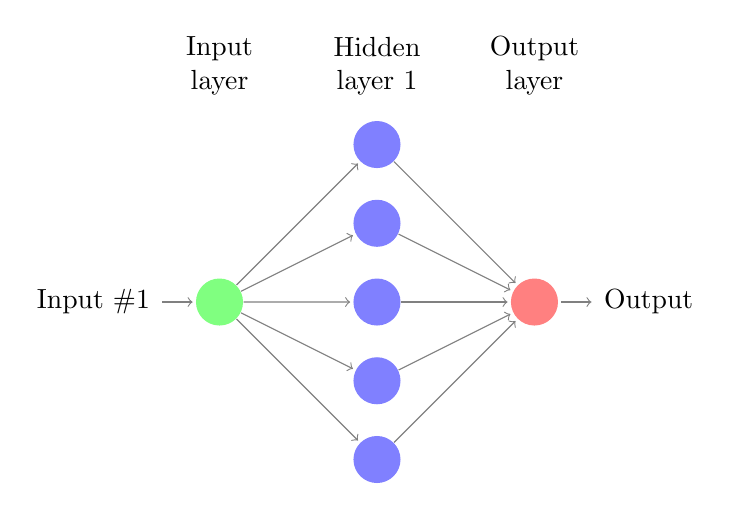
\begin{tikzpicture}[shorten >=1pt,->,draw=black!50, node distance=\layersep]
\tikzstyle{every pin edge}=[<-,shorten <=1pt]
\tikzstyle{neuron}=[circle,fill=black!25,minimum size=17pt,inner sep=0pt]
\tikzstyle{input neuron}=[neuron, fill=green!50];
\tikzstyle{output neuron}=[neuron, fill=red!50];
\tikzstyle{hidden neuron}=[neuron, fill=blue!50];
\tikzstyle{annot} = [text width=4em, text centered]

% Draw the input layer nodes
%   \foreach \name / \y in {1,...,4}
% This is the same as writing \foreach \name / \y in {1/1,2/2,3/3,4/4}
\node[input neuron, pin=left:Input \#1] (I1) at (0,-2.5cm) {};

% Draw the hidden layer nodes
\foreach \name / \y in {1,...,5}
\path[yshift=0.5cm]
node[hidden neuron] (H1-\name) at (\layersep,-\y cm) {};



% Draw the output layer node
\node[output neuron,pin={[pin edge={->}]right:Output}, right of=H1-3] (O) {};

% Connect every node in the input layer with every node in the
% hidden layer.
\foreach \dest in {1,...,5}
\path (I1) edge (H1-\dest);


% Connect every node in the hidden layer with the output layer
\foreach \source in {1,...,5}
\path (H1-\source) edge (O);

% Annotate the layers
\node[annot,above of=H1-1, node distance=1cm] (hl) {Hidden layer 1};
\node[annot,left of=hl] {Input layer};
\node[annot,right of=hl] {Output layer};
\end{tikzpicture}
\caption{Feed-forward neural network for 1D function approximation}
\end{figure}


\begin{figure}
\centering
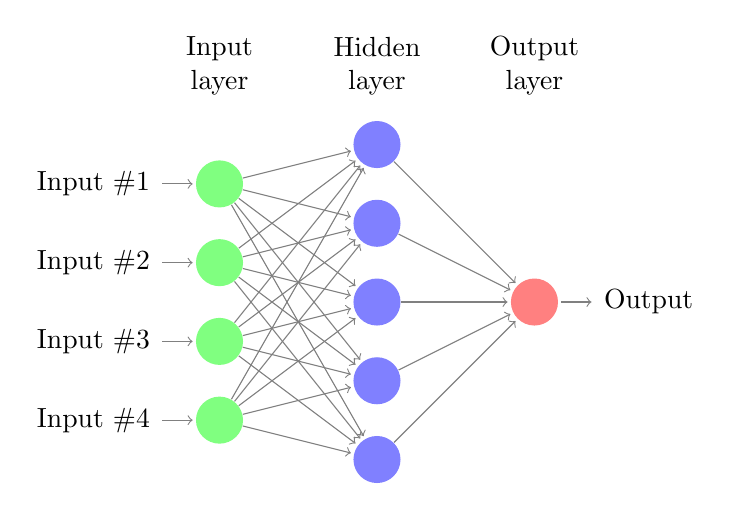
\begin{tikzpicture}[shorten >=1pt,->,draw=black!50, node distance=\layersep]
\tikzstyle{every pin edge}=[<-,shorten <=1pt]
\tikzstyle{neuron}=[circle,fill=black!25,minimum size=17pt,inner sep=0pt]
\tikzstyle{input neuron}=[neuron, fill=green!50];
\tikzstyle{output neuron}=[neuron, fill=red!50];
\tikzstyle{hidden neuron}=[neuron, fill=blue!50];
\tikzstyle{annot} = [text width=4em, text centered]

% Draw the input layer nodes
\foreach \name / \y in {1,...,4}
% This is the same as writing \foreach \name / \y in {1/1,2/2,3/3,4/4}
\node[input neuron, pin=left:Input \#\y] (I-\name) at (0,-\y) {};

% Draw the hidden layer nodes
\foreach \name / \y in {1,...,5}
\path[yshift=0.5cm]
node[hidden neuron] (H-\name) at (\layersep,-\y cm) {};

% Draw the output layer node
\node[output neuron,pin={[pin edge={->}]right:Output}, right of=H-3] (O) {};

% Connect every node in the input layer with every node in the
% hidden layer.
\foreach \source in {1,...,4}
\foreach \dest in {1,...,5}
\path (I-\source) edge (H-\dest);

% Connect every node in the hidden layer with the output layer
\foreach \source in {1,...,5}
\path (H-\source) edge (O);

% Annotate the layers
\node[annot,above of=H-1, node distance=1cm] (hl) {Hidden layer};
\node[annot,left of=hl] {Input layer};
\node[annot,right of=hl] {Output layer};
\end{tikzpicture}
\caption{Feed-forward neural network for 4D function approximation}
\end{figure}

\subsection{Feed-forward neural network for classification}


\section{Notes on Bibliography}

Book \cite{goodfellow2016deep}.

Natural language processing, see \cite{manning1999foundations}
Resources: \href{http://ttic.uchicago.edu/~shubhendu/Pages/CMSC35246.html}{Chicago}

\printbibliography
\end{refsection}
